\documentclass[conference]{IEEEtran}
\IEEEoverridecommandlockouts

\usepackage[T1]{fontenc}
\usepackage{graphicx}
\usepackage{amsmath,amssymb}
\usepackage{booktabs}
\usepackage{tabularx}
\usepackage{multirow}
\usepackage{cite}
\usepackage{url}
\usepackage[hidelinks]{hyperref}
\usepackage{algorithm}
\usepackage{algorithmic}
\usepackage{tikz}
\usetikzlibrary{arrows.meta,positioning,shapes.geometric,calc,fit}

% Make the document build in Overleaf (paper_ieee/ only) and in-repo.
\graphicspath{{figures/}{../results/}{results/}}
\newcommand{\inputtable}[1]{%
  \IfFileExists{tables/#1}{\input{tables/#1}}{\input{paper_ieee/tables/#1}}%
}
\newcommand{\includeresult}[2][]{%
  \IfFileExists{figures/#2}{\includegraphics[#1]{figures/#2}}{%
    \IfFileExists{../results/#2}{\includegraphics[#1]{../results/#2}}{\includegraphics[#1]{results/#2}}%
  }%
}

\title{Adversarial Attacks on GCN and GAT for Node Classification\\and Ontology-Guided Defenses}

\author{
\IEEEauthorblockN{EaswarKrishna A P}
\IEEEauthorblockA{
Department of Network Engineering\\
India\\
email: (omitted for anonymized draft)
}}

\begin{document}
\maketitle

\begin{abstract}
Graph Neural Networks (GNNs) achieve strong results on node classification by repeatedly aggregating information from graph neighborhoods. However, this same message-passing mechanism creates an amplified attack surface: small perturbations to edges or node features can propagate across layers and significantly degrade predictions. This paper presents a complete experimental framework to study adversarial attacks on two canonical architectures, the two-layer Graph Convolutional Network (GCN) and Graph Attention Network (GAT), on both a static benchmark (Cora) and a dynamic evolving-graph generator. We implement three poisoning attacks (random structure corruption, Nettack, and a meta-learning style poisoning attack) and three evasion attacks (degree-preserving edge flips, feature-space evasion, and a gradient-based FGSM-like feature attack). We then evaluate filtering and smoothing defenses (feature smoothing and similarity-based edge pruning) and propose an ontology-guided defense that constructs a semantic similarity matrix from feature-label affinity and feature co-occurrence to reweight aggregation and project features toward consistent subspaces. Across our runs, gradient-aligned feature evasion is the most damaging attack, while the combined pruning+ontology defense recovers a substantial portion of lost accuracy and macro-F1. The project is fully reproducible and outputs metric tables and diagnostic figures.
\end{abstract}

\begin{IEEEkeywords}
Graph Neural Networks, adversarial machine learning, node classification, poisoning attacks, evasion attacks, robustness, ontology-based defense.
\end{IEEEkeywords}

\section{Introduction}
Graph Neural Networks (GNNs) extend deep learning to relational data by learning representations that depend on graph connectivity and neighborhood context. In node classification, this message passing mechanism aggregates information from neighboring nodes and progressively refines embeddings. Yet message passing also creates a failure mode: if an adversary slightly modifies the graph or node attributes, these perturbations can be amplified across layers and lead to large drops in downstream performance.

This paper documents a production-grade experimental framework that implements (i) two-layer GCN and GAT models~\cite{kipf2017gcn,velickovic2018gat}, (ii) representative poisoning and evasion attacks~\cite{zugner2018nettack,zugner2019metattack,goodfellow2015fgsm}, (iii) base-paper-inspired defenses such as similarity-based pruning and feature smoothing~\cite{wu2019jaccard,zhang2020gnnguard}, and (iv) an ontology-guided defense that enforces semantic consistency for robust message passing. The paper is aligned with the robustness literature: it defines a threat model, reports multiple metrics (accuracy/F1/ROC-AUC, ASR, margin drop, log-loss), and includes qualitative diagnostics (confusion matrices, embeddings, and layer-wise outputs).

\textbf{Contributions.} We make four practical contributions:
\begin{itemize}
\item An end-to-end system (training, attacks, defenses, evaluation, visualization) with reproducible seeds and on-disk artifacts.
\item Implementations of six attacks spanning poisoning and evasion, with budgets enforced at the operator level.
\item A defense stack evaluated in three modes (pruning-only, ontology-only, pruning+ontology) against the most impactful attack (largest accuracy drop).
\item A research-paper-ready reporting pipeline: terminal tables, CSV tables, and publishable figures for interpretability.
\end{itemize}

\begin{figure*}[t]
\centering
\resizebox{\textwidth}{!}{%
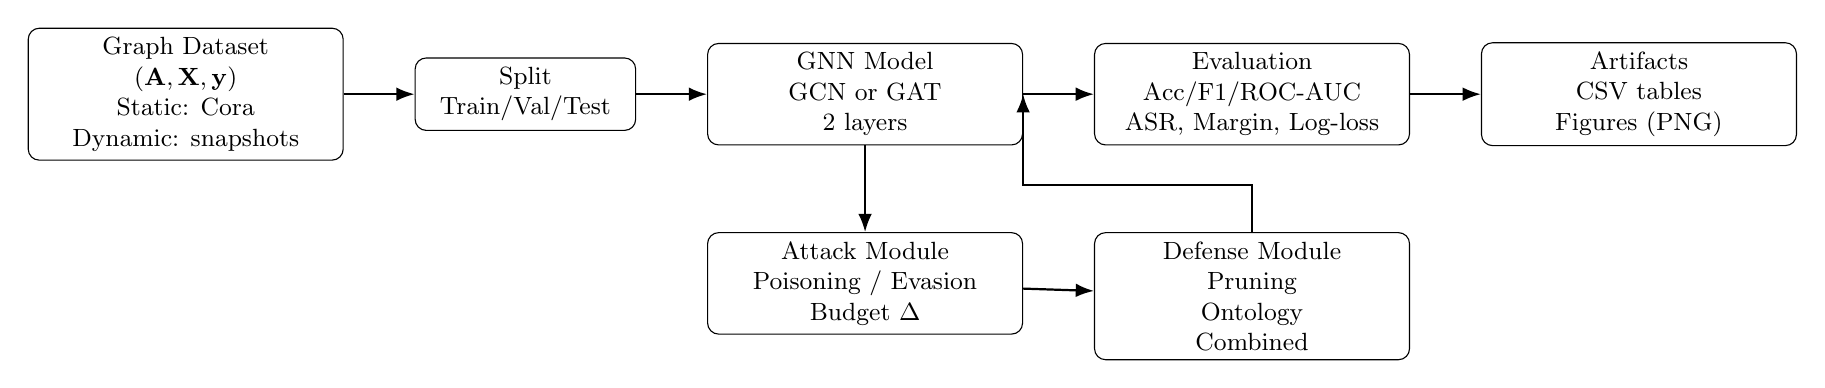
\begin{tikzpicture}[
  font=\small,
  box/.style={draw, rounded corners, align=center, minimum height=9mm, minimum width=28mm},
  big/.style={draw, rounded corners, align=center, minimum height=11mm, minimum width=40mm},
  arrow/.style={-Latex, thick}
]
\node[big] (data) {Graph Dataset\\$(\mathbf{A},\mathbf{X},\mathbf{y})$\\Static: Cora\\Dynamic: snapshots};
\node[box, right=9mm of data] (split) {Split\\Train/Val/Test};
\node[big, right=9mm of split] (model) {GNN Model\\GCN or GAT\\2 layers};
\node[big, right=9mm of model] (eval) {Evaluation\\Acc/F1/ROC-AUC\\ASR, Margin, Log-loss};
\node[big, right=9mm of eval] (art) {Artifacts\\CSV tables\\Figures (PNG)};

\node[big, below=11mm of model] (attack) {Attack Module\\Poisoning / Evasion\\Budget $\Delta$};
\node[big, below=11mm of eval] (def) {Defense Module\\Pruning\\Ontology\\Combined};

\draw[arrow] (data) -- (split);
\draw[arrow] (split) -- (model);
\draw[arrow] (model) -- (eval);
\draw[arrow] (eval) -- (art);
\draw[arrow] (model) -- (attack);
\draw[arrow] (attack) -- (def);
\draw[arrow] (def.north) -- ++(0,6mm) -| (model.east);
\end{tikzpicture}
}%
\caption{End-to-end workflow. Attacks either modify training-time data (poisoning) or inference-time inputs (evasion). Defenses are evaluated individually (pruning-only, ontology-only) and in combination (pruning+ontology) against the most impactful attack.}
\label{fig:workflow}
\end{figure*}

\section{Related Work}
Adversarial machine learning in continuous domains has a large body of work on $\ell_p$-bounded perturbations. Graphs introduce additional complexity due to discrete structure and non-i.i.d. dependencies. Graph adversarial attacks can be categorized into \textit{poisoning} (training-time) and \textit{evasion} (test-time) attacks~\cite{zugner2018nettack,zugner2019metattack}. Nettack~\cite{zugner2018nettack} selects edge and feature modifications that reduce the target margin while maintaining plausibility. Meta-learning based poisoning attacks~\cite{zugner2019metattack} treat perturbations as parameters optimized through training dynamics.

Defenses are commonly split into preprocessing and model-based methods. Similarity-based edge filtering and feature smoothing reduce the impact of suspicious edges/features~\cite{wu2019jaccard}. Low-rank defenses filter adjacency via truncated SVD~\cite{entezari2020svd}. GNNGuard~\cite{zhang2020gnnguard} uses feature similarity to estimate neighbor importance and suppress messages along likely adversarial edges. Our ontology-guided defense uses the same high-level principle (semantic consistency) but implements it as an explicit ontology matrix used for both adjacency reweighting and feature projection.

\section{Methodology}
\subsection{System Pipeline}
The framework follows a consistent pipeline across datasets and threat models: (i) load and preprocess the graph, (ii) train a baseline GCN/GAT, (iii) generate an attacked graph or attacked features under a budget, (iv) evaluate attack impact with classification and robustness metrics, (v) identify the most impactful attack by accuracy drop, and (vi) evaluate defenses individually and in combination against that attack. Every stage produces artifacts (CSV tables and figures) to enable auditability and paper-ready reporting.

\begin{figure*}[t]
\centering
\includeresult[width=0.95\textwidth]{system_flow.png}
\caption{Implementation pipeline rendered from project outputs: dataset loading, baseline training, attack generation (poisoning and evasion), metric evaluation, defenses (pruning/smoothing/ontology), and visualization outputs.}
\label{fig:system_flow}
\end{figure*}

\subsection{Evaluation Metrics}
We report standard metrics (accuracy and macro/micro-F1) and robustness-oriented diagnostics. For a node $i$ with true class $y_i$, we define the \textit{classification margin} as:
\begin{equation}
m_i = Z_{i,y_i} - \max_{c\neq y_i} Z_{i,c},
\end{equation}
where $Z_{i,c}$ is the predicted probability for class $c$. Attacks aim to reduce the margin. We report \textit{margin drop} as the difference in average margin between clean and attacked settings. We also report \textit{attack success rate} (ASR) as the fraction of test nodes whose predicted label changes from correct to incorrect under the attack (implementation: computed from baseline vs attacked predictions under the same test mask for evasion, and via retrained models for poisoning).

\subsection{Selecting the Most Impactful Attack}
For each model, we compute accuracy drop relative to the baseline:
\begin{equation}
\Delta_{\mathrm{acc}}(\mathcal{A}) = \mathrm{Acc}_{\mathrm{base}} - \mathrm{Acc}_{\mathcal{A}}.
\end{equation}
The most impactful attack is $\arg\max_{\mathcal{A}} \Delta_{\mathrm{acc}}(\mathcal{A})$. Defenses are then evaluated against that attack to avoid cherry-picking.

\section{Background and Problem Formulation}
\subsection{Notation}
Let $\mathcal{G}=(\mathcal{V},\mathcal{E})$ be a graph with $N=|\mathcal{V}|$ nodes. $\mathbf{A}\in\{0,1\}^{N\times N}$ is the adjacency matrix and $\mathbf{X}\in\mathbb{R}^{N\times F}$ the node feature matrix. The label vector is $\mathbf{y}\in\{1,\dots,C\}^{N}$ for $C$ classes. We use self-loops $\hat{\mathbf{A}}=\mathbf{A}+\mathbf{I}$ and $\hat{\mathbf{D}}$ as the degree matrix of $\hat{\mathbf{A}}$.

\subsection{Two-Layer GCN}
The two-layer GCN~\cite{kipf2017gcn} uses symmetric normalization $\tilde{\mathbf{A}}=\hat{\mathbf{D}}^{-1/2}\hat{\mathbf{A}}\hat{\mathbf{D}}^{-1/2}$:
\begin{align}
\mathbf{H}^{(1)} &= \mathrm{ReLU}(\tilde{\mathbf{A}}\mathbf{X}\mathbf{W}^{(0)}), \label{eq:gcn1}\\
\mathbf{Z} &= \mathrm{softmax}(\tilde{\mathbf{A}}\mathbf{H}^{(1)}\mathbf{W}^{(1)}), \label{eq:gcn2}
\end{align}
where $\mathbf{W}^{(0)}\in\mathbb{R}^{F\times H}$ and $\mathbf{W}^{(1)}\in\mathbb{R}^{H\times C}$.

\subsection{Two-Layer GAT}
GAT~\cite{velickovic2018gat} uses attention coefficients on edges $(i,j)$:
\begin{align}
e_{ij} &= \mathrm{LeakyReLU}\big(\mathbf{a}^\top[\mathbf{W}\mathbf{h}_i \,\|\, \mathbf{W}\mathbf{h}_j]\big), \\
\alpha_{ij} &= \mathrm{softmax}_j(e_{ij})=\frac{\exp(e_{ij})}{\sum_{k\in\mathcal{N}(i)}\exp(e_{ik})}, \\
\mathbf{h}'_i &= \sum_{j\in\mathcal{N}(i)}\alpha_{ij}\mathbf{W}\mathbf{h}_j .
\end{align}
We use multi-head attention (4 heads) in the hidden layer with ELU activation, followed by a softmax output layer.

\begin{figure*}[t]
\centering
\resizebox{\textwidth}{!}{%
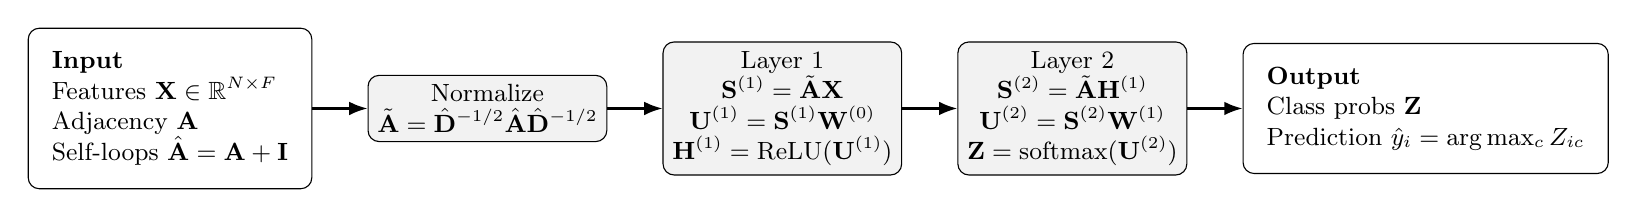
\begin{tikzpicture}[
  font=\small,
  box/.style={draw, rounded corners, align=left, minimum height=8mm, inner sep=3mm},
  op/.style={draw, rounded corners, fill=gray!10, align=center, minimum height=8mm, minimum width=28mm},
  arrow/.style={-Latex, thick}
]
\node[box] (in) {\textbf{Input}\\Features $\mathbf{X}\in\mathbb{R}^{N\times F}$\\Adjacency $\mathbf{A}$\\Self-loops $\hat{\mathbf{A}}=\mathbf{A}+\mathbf{I}$};
\node[op, right=7mm of in] (norm) {Normalize\\$\tilde{\mathbf{A}}=\hat{\mathbf{D}}^{-1/2}\hat{\mathbf{A}}\hat{\mathbf{D}}^{-1/2}$};
\node[op, right=7mm of norm] (l1) {Layer 1\\$\mathbf{S}^{(1)}=\tilde{\mathbf{A}}\mathbf{X}$\\$\mathbf{U}^{(1)}=\mathbf{S}^{(1)}\mathbf{W}^{(0)}$\\$\mathbf{H}^{(1)}=\mathrm{ReLU}(\mathbf{U}^{(1)})$};
\node[op, right=7mm of l1] (l2) {Layer 2\\$\mathbf{S}^{(2)}=\tilde{\mathbf{A}}\mathbf{H}^{(1)}$\\$\mathbf{U}^{(2)}=\mathbf{S}^{(2)}\mathbf{W}^{(1)}$\\$\mathbf{Z}=\mathrm{softmax}(\mathbf{U}^{(2)})$};
\node[box, right=7mm of l2] (out) {\textbf{Output}\\Class probs $\mathbf{Z}$\\Prediction $\hat{y}_i=\arg\max_c Z_{ic}$};
\draw[arrow] (in) -- (norm);
\draw[arrow] (norm) -- (l1);
\draw[arrow] (l1) -- (l2);
\draw[arrow] (l2) -- (out);
\end{tikzpicture}
}%
\caption{Detailed two-layer GCN computation graph used in this project (inputs, per-layer functions, and outputs). The code logs layer-wise tensors (pre-aggregation, post-normalization, post-activation, logits, probabilities) to connect attacks/defenses to internal computations.}
\label{fig:gcn_arch}
\end{figure*}

\subsection{Threat Model}
We consider poisoning attackers that modify the training graph and evasion attackers that only modify inference-time inputs. Attacks are constrained by a budget $\Delta$ (edge flips, feature flips, or an $\ell_\infty$ bound for gradient attacks). The defender may deploy preprocessing and/or training-time defenses.

\section{Attacks}
\subsection{Poisoning Attacks}
\textbf{Random Structure Corruption} rewires a budgeted number of edges uniformly at random (with optional feature corruption) to simulate large-scale non-adaptive perturbations.
\textbf{Nettack}~\cite{zugner2018nettack} greedily selects structure/feature modifications that reduce the target node margin while respecting plausibility constraints.
\textbf{Meta Attack}~\cite{zugner2019metattack} approximates bilevel optimization where the outer objective reflects the trained model loss under perturbations.

\subsection{Evasion Attacks}
\textbf{Evasion Edge Flip} modifies only the target node neighborhood at test-time, approximately preserving degree to isolate localized adjacency edits.
\textbf{Evasion Feature} flips binary feature entries (or adds bounded noise for continuous features) only at inference time; training data remains untouched.
\textbf{FGSM-like Feature Attack} applies a gradient-sign update~\cite{goodfellow2015fgsm}:
\begin{equation}
\mathbf{X}_{adv} = \mathbf{X} + \epsilon\cdot \mathrm{sign}(\nabla_{\mathbf{X}}\mathcal{L}(\mathbf{Z},\mathbf{y})),
\end{equation}
where $\epsilon$ is the perturbation magnitude.

\section{Defenses}
\subsection{Feature Smoothing and Consistency}
We implement Laplacian feature smoothing:
\begin{equation}
\mathbf{X}_{smooth} = \alpha\mathbf{X} + (1-\alpha)\tilde{\mathbf{A}}\mathbf{X},
\end{equation}
and a feature-consistency penalty $\|\mathbf{X}-\tilde{\mathbf{A}}\mathbf{X}\|_2^2$ that encourages neighborhood-consistent signals.

\subsection{Pruning Defense (Similarity Filtering)}
We implement similarity-based pruning inspired by prior work~\cite{wu2019jaccard,zhang2020gnnguard}: edges between feature-dissimilar nodes are down-weighted or removed based on cosine/Jaccard similarity. This mitigates attacks that inject adversarial edges to connect unrelated regions.

\subsection{Ontology-Guided Defense}
We construct an ontology matrix $\mathbf{O}$ from (i) feature co-occurrence similarity and (ii) feature-label affinity on the training set. The defense uses:
\begin{align}
\mathbf{A}' &= (1-\lambda)\mathbf{A}+\lambda\,\psi(\mathbf{O}), \\
\mathbf{X}' &= (1-\lambda)\mathbf{X}+\lambda\,\mathbf{O}\mathbf{X},
\end{align}
where $\psi(\cdot)$ maps semantic affinity to edge weights. This suppresses messages that contradict semantic consistency and dampens adversarial feature edits.

\begin{algorithm}[t]
\caption{Ontology-Guided Defense (Adjacency Reweighting + Feature Projection)}
\label{alg:ontology}
\begin{algorithmic}[1]
\STATE Input: adjacency $\mathbf{A}$, features $\mathbf{X}$, labels $\mathbf{y}$ (train), strength $\lambda$.
\STATE Build ontology matrix $\mathbf{O}$ from feature co-occurrence and feature-label affinity.
\STATE Reweight adjacency: $\mathbf{A}' \leftarrow (1-\lambda)\mathbf{A} + \lambda\,\psi(\mathbf{O})$.
\STATE Project features: $\mathbf{X}' \leftarrow (1-\lambda)\mathbf{X} + \lambda\,\mathbf{O}\mathbf{X}$.
\STATE Train/evaluate GNN on $(\mathbf{A}',\mathbf{X}')$.
\end{algorithmic}
\end{algorithm}

\subsection{Combined Defense}
We evaluate pruning-only, ontology-only, and pruning+ontology. The combined mode first prunes suspicious edges and then applies ontology reweighting/projection to further stabilize message passing.

\section{Semantic Logic Design}
This section clarifies why the proposed ontology-guided defense is \textit{not} equivalent to similarity pruning.
\textbf{Similarity pruning} (e.g., cosine/Jaccard filtering) is purely geometric: it assigns edge trust directly from feature similarity and removes edges below a threshold. It does not define any explicit semantic entities, relations, or constraints, and it cannot express \textit{impossible} feature combinations or cross-topic contradictions.

\textbf{Ontology-guided defense} introduces explicit semantic structure:
\begin{itemize}
\item \textbf{Concepts (classes):} \texttt{ResearchTopic} with dataset-specific topic classes (labels) and subtopics (subclasses).
\item \textbf{Relations (object properties):} \texttt{indicatesTopic} (feature$\rightarrow$topic), \texttt{coOccursWith} (feature$\leftrightarrow$feature), \texttt{contradicts} (feature$\times$feature).
\item \textbf{Attributes (data properties):} affinity score, co-occurrence score, and inheritance score.
\item \textbf{Constraints and rules:} contradiction filtering and repair rules (SWRL-like) that detect semantically impossible combinations and reduce trust for edges/nodes that violate constraints.
\item \textbf{Inheritance:} subtopics inherit parent semantics, enabling graded reasoning rather than hard class boundaries.
\end{itemize}
These symbolic structures drive two numeric signals for robust message passing: (i) semantic edge trust (used to reweight/prune edges) and (ii) semantic feature projection/repair (used to denoise adversarial feature edits). This is a knowledge-guided robustness mechanism, not a local similarity heuristic.

\subsection{Ablation: Which Semantic Logic Helps?}
To avoid unclear contribution sources, we ablate ontology components and report accuracy. The variants correspond to different semantic logic paths (co-occurrence graph only, label affinity only, rules only, projection only, full ontology).
\inputtable{semantic_ablation.tex}

\subsection{Benchmark: SOTA-Style Defense Comparisons}
We benchmark the ontology defense against representative baselines implemented in our framework, including smoothing, GNNGuard-like similarity weighting, low-rank filtering (GNN-SVD), and adversarial training, and we report the best-performing variant per defense.
\inputtable{defense_benchmark.tex}

\section{Experimental Setup}
\subsection{Datasets}
\textbf{Static graph: Cora.} We use the Cora citation network for node classification with sparse bag-of-words features and 7 classes.
\textbf{Dynamic graph: evolving snapshots.} We generate graph snapshots by applying controlled edge additions/removals and feature drift over time, and report aggregated robustness across snapshots.

\subsection{Models and Training}
Both GCN and GAT are instantiated as two-layer networks with dropout and Adam optimization. Poisoning attacks retrain the model on perturbed training data. Evasion attacks evaluate on fixed trained weights (training data unchanged).

\subsection{Metrics}
We report accuracy, macro/micro-F1, ROC-AUC (one-vs-rest), log-loss, attack success rate (ASR), robustness score, perturbation rate, and margin drop. Metrics are printed as terminal tables and written to CSV.

\section{Results}
\subsection{Static Graph: Attack Comparison}
Tables~\ref{tab:static_gcn_attacks} and~\ref{tab:static_gat_attacks} summarize the attack suite on Cora for GCN and GAT (before defenses). Across both models, gradient-aligned feature evasion causes the largest accuracy drop, demonstrating that feature-space perturbations aligned with the loss can overwhelm the decision boundary even when structure is unchanged.

\inputtable{static_gcn_attacks.tex}
\inputtable{static_gat_attacks.tex}

\subsection{Static Graph: Defenses Against the Most Impactful Attack}
Tables~\ref{tab:static_gcn_defenses} and~\ref{tab:static_gat_defenses} report defenses evaluated against the most impactful attack. Pruning and smoothing improve robustness, and ontology-based defenses further improve accuracy and calibration.

\inputtable{static_gcn_defenses.tex}
\inputtable{static_gat_defenses.tex}

\subsection{Qualitative Diagnostics}
We include confusion matrices, t-SNE embeddings, and layer-wise output panels to validate that attacks shift internal representations and that defenses restore structure.

\begin{figure*}[t]
\centering
\includeresult[width=0.95\textwidth]{graph_mosaic.png}
\caption{Local subgraph visualization (clean vs attacked vs defended) from project outputs. Even small perturbations can inject cross-community edges or distort neighborhood feature consistency, which propagates through message passing. Defenses suppress suspicious connections and restore a more coherent neighborhood.}
\label{fig:graph_mosaic}
\end{figure*}

\begin{figure}[t]
\centering
\includeresult[width=0.98\columnwidth]{robustness_curve.png}
\caption{Robustness curve on Cora: accuracy vs. feature-perturbation budget.}
\label{fig:robustness_curve}
\end{figure}

\begin{figure}[t]
\centering
\includeresult[width=0.98\columnwidth]{confusion_baseline.png}\\
\includeresult[width=0.98\columnwidth]{confusion_feature_attack.png}\\
\includeresult[width=0.98\columnwidth]{confusion_ontology_defense.png}
\caption{Confusion matrices on Cora (top: baseline, middle: attacked, bottom: ontology defense).}
\label{fig:confusions}
\end{figure}

\begin{figure*}[t]
\centering
\includeresult[width=0.32\textwidth]{tsne_clean.png}
\includeresult[width=0.32\textwidth]{tsne_attacked.png}
\includeresult[width=0.32\textwidth]{tsne_defended.png}
\caption{t-SNE embeddings from the hidden layer: clean (left), attacked (middle), defended (right).}
\label{fig:tsne}
\end{figure*}

\begin{figure}[t]
\centering
\includeresult[width=0.98\columnwidth]{layer_outputs_gcn.png}
\caption{GCN layer-wise output panel (pre-aggregation, post-normalization, post-activation, logits).}
\label{fig:layer_gcn}
\end{figure}

\begin{figure}[t]
\centering
\includeresult[width=0.98\columnwidth]{layer_outputs_gat.png}
\caption{GAT layer-wise output panel (hidden activations, logits, probabilities).}
\label{fig:layer_gat}
\end{figure}

\subsection{Graph Structural Metrics}
\inputtable{graph_metrics_static.tex}

\subsection{Dynamic Graph Robustness}
\inputtable{dynamic_gcn_summary.tex}
\inputtable{graph_metrics_dynamic.tex}
\inputtable{dynamic_defense_sweep.tex}

\section{Discussion}
Three observations stand out. (1) Gradient-aligned feature attacks dominate in damage, implying defenses must directly address feature integrity. (2) Defenses must preserve utility: over-pruning or over-smoothing can harm clean accuracy. (3) Qualitative diagnostics (embeddings, confusion matrices, layer-wise outputs) help validate that observed accuracy changes correspond to meaningful representation shifts.

\section{Broader Impact and Ethics}
Robustness methods for GNNs can reduce harm in applications such as fraud detection, recommender systems, and knowledge graph analytics where adversaries may manipulate edges or features. Attack implementations are dual-use; this project is intended for research and educational evaluation with controlled budgets and public datasets.

\section{Limitations and Future Work}
The ontology matrix here is derived from available features and labels; integrating external domain ontologies could improve semantic fidelity but requires additional data sources. Evaluations focus on node classification; extending to link prediction or graph classification would test generality. Future work should also explore stronger black-box attackers and systematic hyperparameter searches for defense tuning.

\section{Conclusion}
We presented an end-to-end framework to study adversarial attacks on GCN and GAT for node classification and evaluated defenses including feature smoothing, pruning, and an ontology-guided semantic defense. On Cora and dynamic graph snapshots, gradient-based feature evasion is the most damaging attack, while pruning+ontology defenses recover a substantial portion of performance and improve calibration. The repository includes full artifacts suitable for reproducible research.

\appendices
\section{Reproducibility and Artifacts}
All experiments write CSV tables and PNG figures to the project \texttt{results/} directory. The LaTeX report references these artifacts directly.

\section{Ontology Construction Details}
The ontology matrix $\mathbf{O}$ is constructed by combining (i) a feature co-occurrence similarity matrix (cosine similarity in feature space) and (ii) a feature-label affinity matrix estimated from the training set. The combination weight is a hyperparameter. This design aims to approximate topic-level semantics in citation graphs without requiring external knowledge bases.

\section{Attack Implementation Notes}
This appendix summarizes how each attack is realized in code to match the threat model.
\textbf{Poisoning attacks} output a modified training graph and trigger retraining. Random structure corruption flips a large number of edges and optionally corrupts a small subset of features. Nettack selects candidate perturbations that reduce the target margin while preserving basic constraints (e.g., sparsity and feature validity). Meta attack approximates bilevel optimization by taking gradient steps on a relaxed perturbation representation and then discretizing.
\textbf{Evasion attacks} keep the trained model fixed. Evasion edge flip edits only the target neighborhood with a small budget and aims to preserve degree distribution. Evasion feature flips a bounded number of binary feature indices for selected nodes, and the FGSM-like attack computes $\nabla_{\mathbf{X}}\mathcal{L}$ on the current model and applies an $\ell_\infty$-bounded sign update.

\section{Defense Hyperparameters}
Defenses introduce tuning parameters. Smoothing uses $\alpha\in[0,1]$; pruning uses a similarity threshold $\tau$ and a metric choice (cosine or Jaccard); ontology uses $\lambda\in[0,1]$ and a semantic weighting factor that trades off feature co-occurrence vs label affinity. In the experiments, we report a hyperparameter sweep for the dynamic setting to show the stability of results across reasonable ranges.

\section{Dynamic Graph Generator}
The dynamic dataset is a synthetic evolving-graph stream producing snapshots $\{\mathcal{G}_t\}_{t=1}^T$. Each step perturbs adjacency by adding/removing edges under a small rate and applies feature drift by injecting bounded noise into a subset of nodes. This generator provides a controlled testbed for robustness under distribution shift and evolving neighborhoods.

\bibliographystyle{IEEEtran}
\bibliography{refs}

\end{document}
